\chapter{Description of the input files\label{chap:general}}
%-----------------------------------------------------------

\lettrine[lines=2, loversize=0.0, lraise=0.5]{T}{he} input files required by \diva for simple 2-D analysis are described here. input files required by \diva for simple 2-D analysis are described here.
input files required by \diva for simple 2-D analysis are described here.




\minitoc

\newpage % 




%
%Only three files are needed as input:
%
%\begin{enumerate}
%\item a file containing the data (\texttt{data.dat})
%\item the specification of the domain of analysis (\texttt{coast.cont}) and 
%\item the list of the parameters used during the analysis (\texttt{param.par}).
%\end{enumerate}

\begin{center}
\fbox{
\begin{minipage}{0.9\textwidth}
\vspace{.25cm}
\textbf{Convention:} \diva\, works with decimal numbers represented with\quad \textbf{.}\quad  not \textbf{,}\quad

If you use excel for exporting data, try to respect the convention if possible. 
\vspace{.25cm}
\end{minipage}
}
\end{center}


\btips

Use editor \textsl{vi} (see Sec. \ref{sec:vi}) to perform this task.

Simply type:

%\begin{verbatim}
%vi topo.gebco
%:,$s/,/./g
%\end{verbatim}
\etips


\btips

If you do not like \texttt{vi}, you can use the following batch command:
\begin{verbatim}
cat file1 | sed s/,/./g > file2
\end{verbatim}

where: \texttt{file1} is the old file and \\
\hphantom{where:} \texttt{file2} is the file where the replacement has been made.
\etips




\section{Data}
%----------------

The data file contains three (or four) columns: \texttt{ X | Y | value | (relative weight)}.\\
If the number of column is three, the fourth column is assumed to take the value $1$. If there are more than four columns, columns 5 and higher are not used by the software.% (but can be used by the user) .

\begin{figure}[H]
\centering

\parbox{.5\textwidth}{
\begin{footnotesize}
\tt
--------\\
25 25	5\\
25 75 10\\
75 75 5\\
75 25 10\\
--------
\end{footnotesize}
}\parbox{.5\textwidth}{
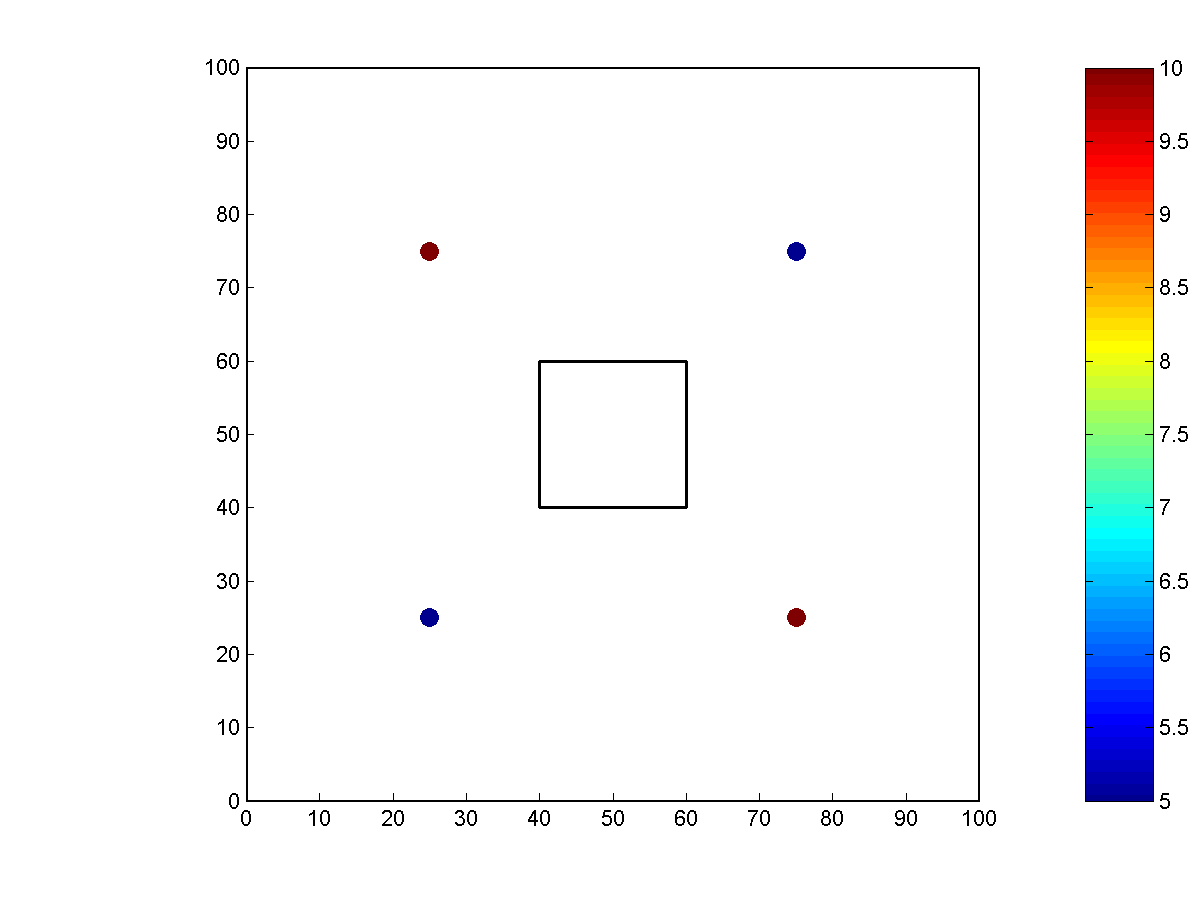
\includegraphics[width=.45\textwidth]{island_data}
}
\caption{Example of a data file and its graphical representation.}
\end{figure}


\section{Contour\label{contourdiva}}
%--------------------------------------

The contour files are defined this way:
\begin{enumerate}
\item The first line indicates the number of contours in the region of interest (say $M$).
\item The second line tells the number of points in the first contour (say $N_{1}$).
\item The next $N_1$ lines are the coordinates of the points of the first contour. The convention for the contour is that \textsl{the land is on the right when you follow the points successively}. The contour is automatically closed, meaning that the last point of a given contour should be different from the first one. 
\item The following line is the number of points of the second contour (say $N_{2}$).
\item \ldots
\item The last $N_M$ lines are the coordinates of the points of the last contour.
\end{enumerate}


\begin{figure}[H]
\centering 
\parbox{.5\textwidth}{

\begin{footnotesize}
\tt
--------\\
2\\
4\\
0 0\\
100 0\\
100 100\\
0 100\\
4\\
40 40\\
40 60\\
60 60\\
60 40\\
--------
\end{footnotesize}

}\parbox{.5\textwidth}{
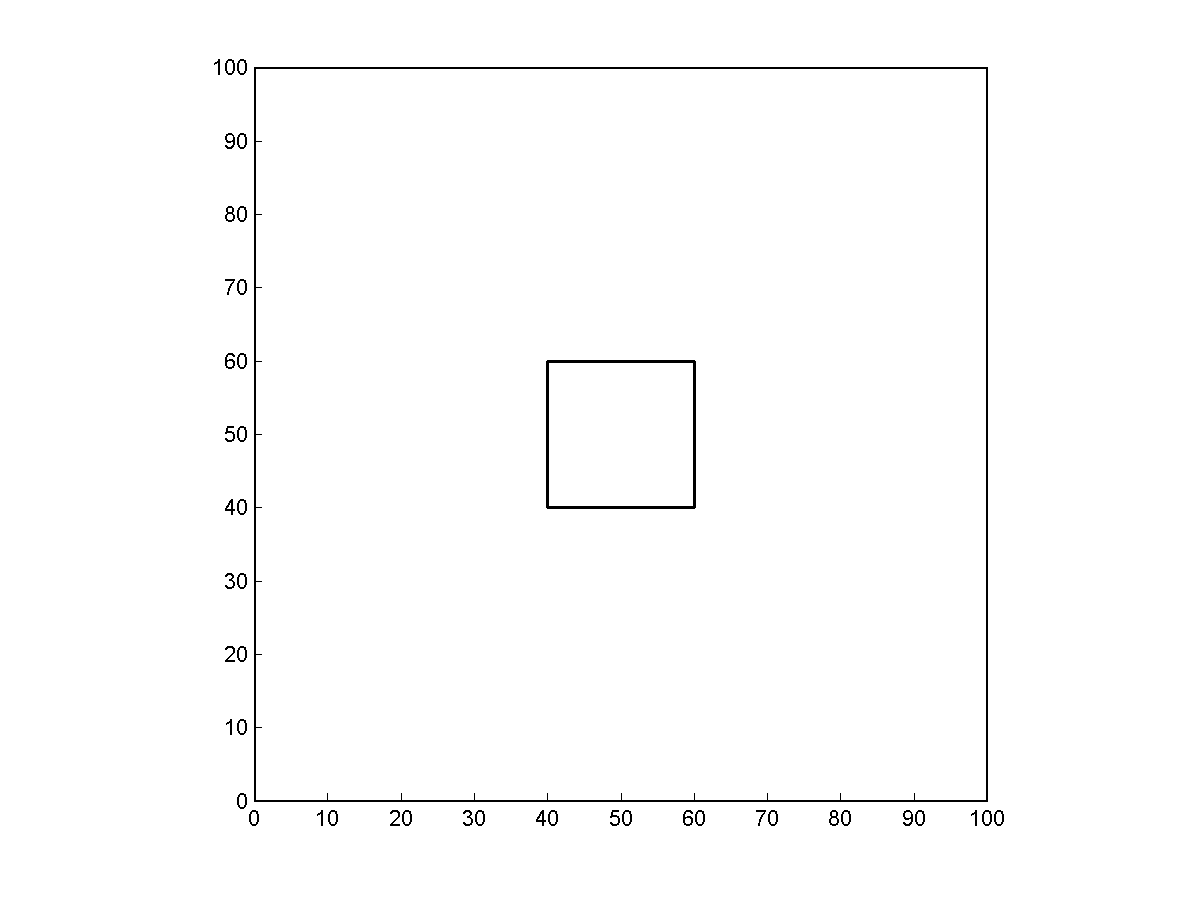
\includegraphics[width=.45\textwidth]{island_contour}
}

\caption{Example of a contour file and its graphical representation.}
\end{figure}



\section[Additional points of analysis]{Locations of additional points where analysis is required (optional)}
%--------------------------------------------------------------------------------

The file \texttt{valatxy.coord} is a two-column list of locations where you want the analysis to be performed.  

\begin{exfile}[htpb]
\begin{footnotesize}
\texttt{-5 0\\
-4.7436 0\\
-4.4872 0\\
-4.2308 0\\
-3.9744 0\\
-3.7179 0\\
-3.4615 0} 
\end{footnotesize}
\caption{valatxy.coord\label{ex:valatxy}}
\end{exfile}

If there are more than two columns, columns 3 and higher are not used.

\section{Parameters\label{sec:param.par}}
%-------------------------------------------

In each step of a \diva\, analysis, many parameters can be changed according to the particular case you are treating. If you work with the CL version, these parameters have to be entered in the file \texttt{param.par} (see file \ref{paramfile}). If you work with the GUI version, the parameters are chosen one after each other during the analysis.

Here is a example of a \texttt{param.par} file followed by the description of all the parameters.

\begin{exfile}[htpb]
\begin{footnotesize}
\begin{verbatim}
# Lc: correlation length (in units coherent with your data)
10
# icoordchange (=0 if no change of coordinates is to be performed (...)
1
# ispec (output files required)
3
# ireg (mode selected for background field: 0=null guess;         (...)
1
# xori: x-coordinate of the first grid point of the output
15
# yori: y-coordinate of the first grid point of the output
66
# dx: step of output grid
0.2
# dy: step of output grid
0.05
# nx: number of grid points in the x-direction
300
# ny: number of grid points in the y-direction
300
# valex (exclusion value)
-999.0
# snr signal to noise ratio of the whole dataset
30
# varbak: variance of the background field. If zero,              (...)
0
\end{verbatim}
\end{footnotesize}
\caption{param.par\label{paramfile}}
\end{exfile}



\subsection{\texttt{Lc}}
% ------------------------

Global correlation length used for the analysis (see Sec. \ref{sec:parammeaning} for the physical meaning).

\subsection{\texttt{icoordchange}\label{sec:icoord}}
%---------------------------------------------------


Specifies the desired type of coordinate system:\\

\texttt{icoordchange} \begin{minipage}[t]{.7\textwidth} = $0$ if no change is necessary (data position in kilometers);\\
                                                        = $1$ if data positions are given in degrees;\\
                                                        = $2$ if data positions are given in degrees and your domain extends on a wide span of latitude                                                           (uses a cosine projection);\\
                                                        = $-xscale$ to scale $x$ coordinates by $xscale$ before doing anything ( for vertical                                                              sections)
                      \end{minipage}
                      
                      
\subsection{\texttt{ispec}}
%--------------------------

Four base-values specifies the required error outputs:\\

\texttt{ispec}       = 0\qquad: no error field requested\\
\hphantom{\texttt{ispec}}  = 1\qquad: gridded error field specified by \texttt{xori}, \texttt{yori}, \texttt{nx} and \texttt{ny}; \\
\hphantom{\texttt{ispec}}  = 2\qquad: errors at data locations;\\
\hphantom{\texttt{ispec}}  = 4\qquad: errors at locations listed in \texttt{valatxy.coord}.

Then you can combine these four values to obtain several error outputs:

\examples\\
\texttt{ispec}             = 3 (=1+2)\hphantom{+4} \qquad \begin{minipage}[t]{.7\textwidth}means you want gridded error field as well as errors at data locations;\end{minipage}\\ 
\texttt{ispec}             = 7 (=1+2+4) \qquad means you want the three error files.


For computing errors with the real covariance function, %(Sec. \ref{})
simply multiply the \texttt{ispec} value by $-1$:

\example\\
\texttt{ispec}             = -7 \qquad \begin{minipage}[t]{.7\textwidth}{means you want the three error files computed with the help of the real covariance function.}\end{minipage}


Finally, a \textit{poor man's} error estimate (quick and underestimated error field) is available by adding $+10$ to the \texttt{ispec} value:

\example\\
\texttt{ispec}             = 16 \qquad \begin{minipage}[t]{.7\textwidth}{means you want errors at data locations and at points listed in \texttt{valatxy.coord} computed with the \textit{poor man's} error estimate.}\end{minipage}


\subsection{\texttt{ireg}}

Specification of the background field which is subtracted from the data field (Sec. \ref{sec:backgroundfield}).

\texttt{ireg}             = 0\qquad: no background field is subtracted (assuming data are already anomalies); \\
\hphantom{\texttt{ireg}}  = 1 \qquad: the data mean value is subtracted;\\
\hphantom{\texttt{ireg}}  = 2 \qquad: the linear regression of the data (plane) is subtracted.

\subsection{\texttt{xori/yori, nx/ny}}

\texttt{xori/yori} indicate the coordinates of the first grid point while \texttt{nx/ny} indicate the number of grid points in \texttt{x/y} directions.



\subsection{\texttt{valex}}
%-----------------------------

Exclusion value: value used to fill the output matrix when a point corresponds with land.


\subsection{\texttt{snr}}
%---------------------------

Signal-to-noise ratio of the whole dataset (Sec. \ref{sec:formulation}).


\subsection{\texttt{varbak}}
%------------------------------

Variance of the background field.


%\subsection{Other parameters} 
%%----------------------------
%The GUI gives the user the possibility to chose the value of parameters:
%
%\begin{itemize}
%\item Surface coefficient: controls the shape of the triangular element.
%\item Smooth number: controls smoothing of the mesh elements.
%\end{itemize}

\section{Working directories}
% ------------------------------

The Command Line version is contained in \texttt{diva-\divaversion/divastripped}. Four subdirectories exist inside \texttt{divastripped}:

\begin{enumerate}
\item \texttt{input} contains data, contour(s) and parameters needed by \diva\, to perform an analysis.

\item \texttt{meshgenwork} is the mesh generation working directory.

\item \texttt{divawork} is the working directory of the CL version, where the \diva\, calculation is performed. 

\item \texttt{output} contains user results.

\item \texttt{gnuwork} is used for quick visualisation with gnuplot.

\end{enumerate}
